
\section{Metrics}
\label{sec:metrics}

% We follow the evaluation protocol of Interp3D~\cite{liu2026interp3d}, reporting 

Commonly, to evaluate 3D morphing the following metrics are employed: FID~\cite{heusel2017fid} to evaluate the distribution of generated states, perceptual path length (PPL)~\cite{karras2019stylegan} to measure the accumulated perceptual variation along the morphing trajectory, and perceptual distance variance (PDV)~\cite{zhang2024diffmorpher} to measure the variability of perceptual distances between consecutive states. While these metrics characterize image quality and different properties of the morphing path, they do not explicitly evaluate how the generated states progress relative to the two sources. For this reason, we introduce and evaluate source-relative progression through Source Profile Error (SPE).

\subsection{Source Profile Error}
\label{sec:spe}

% \begin{figure}[t]
%     \centering
%     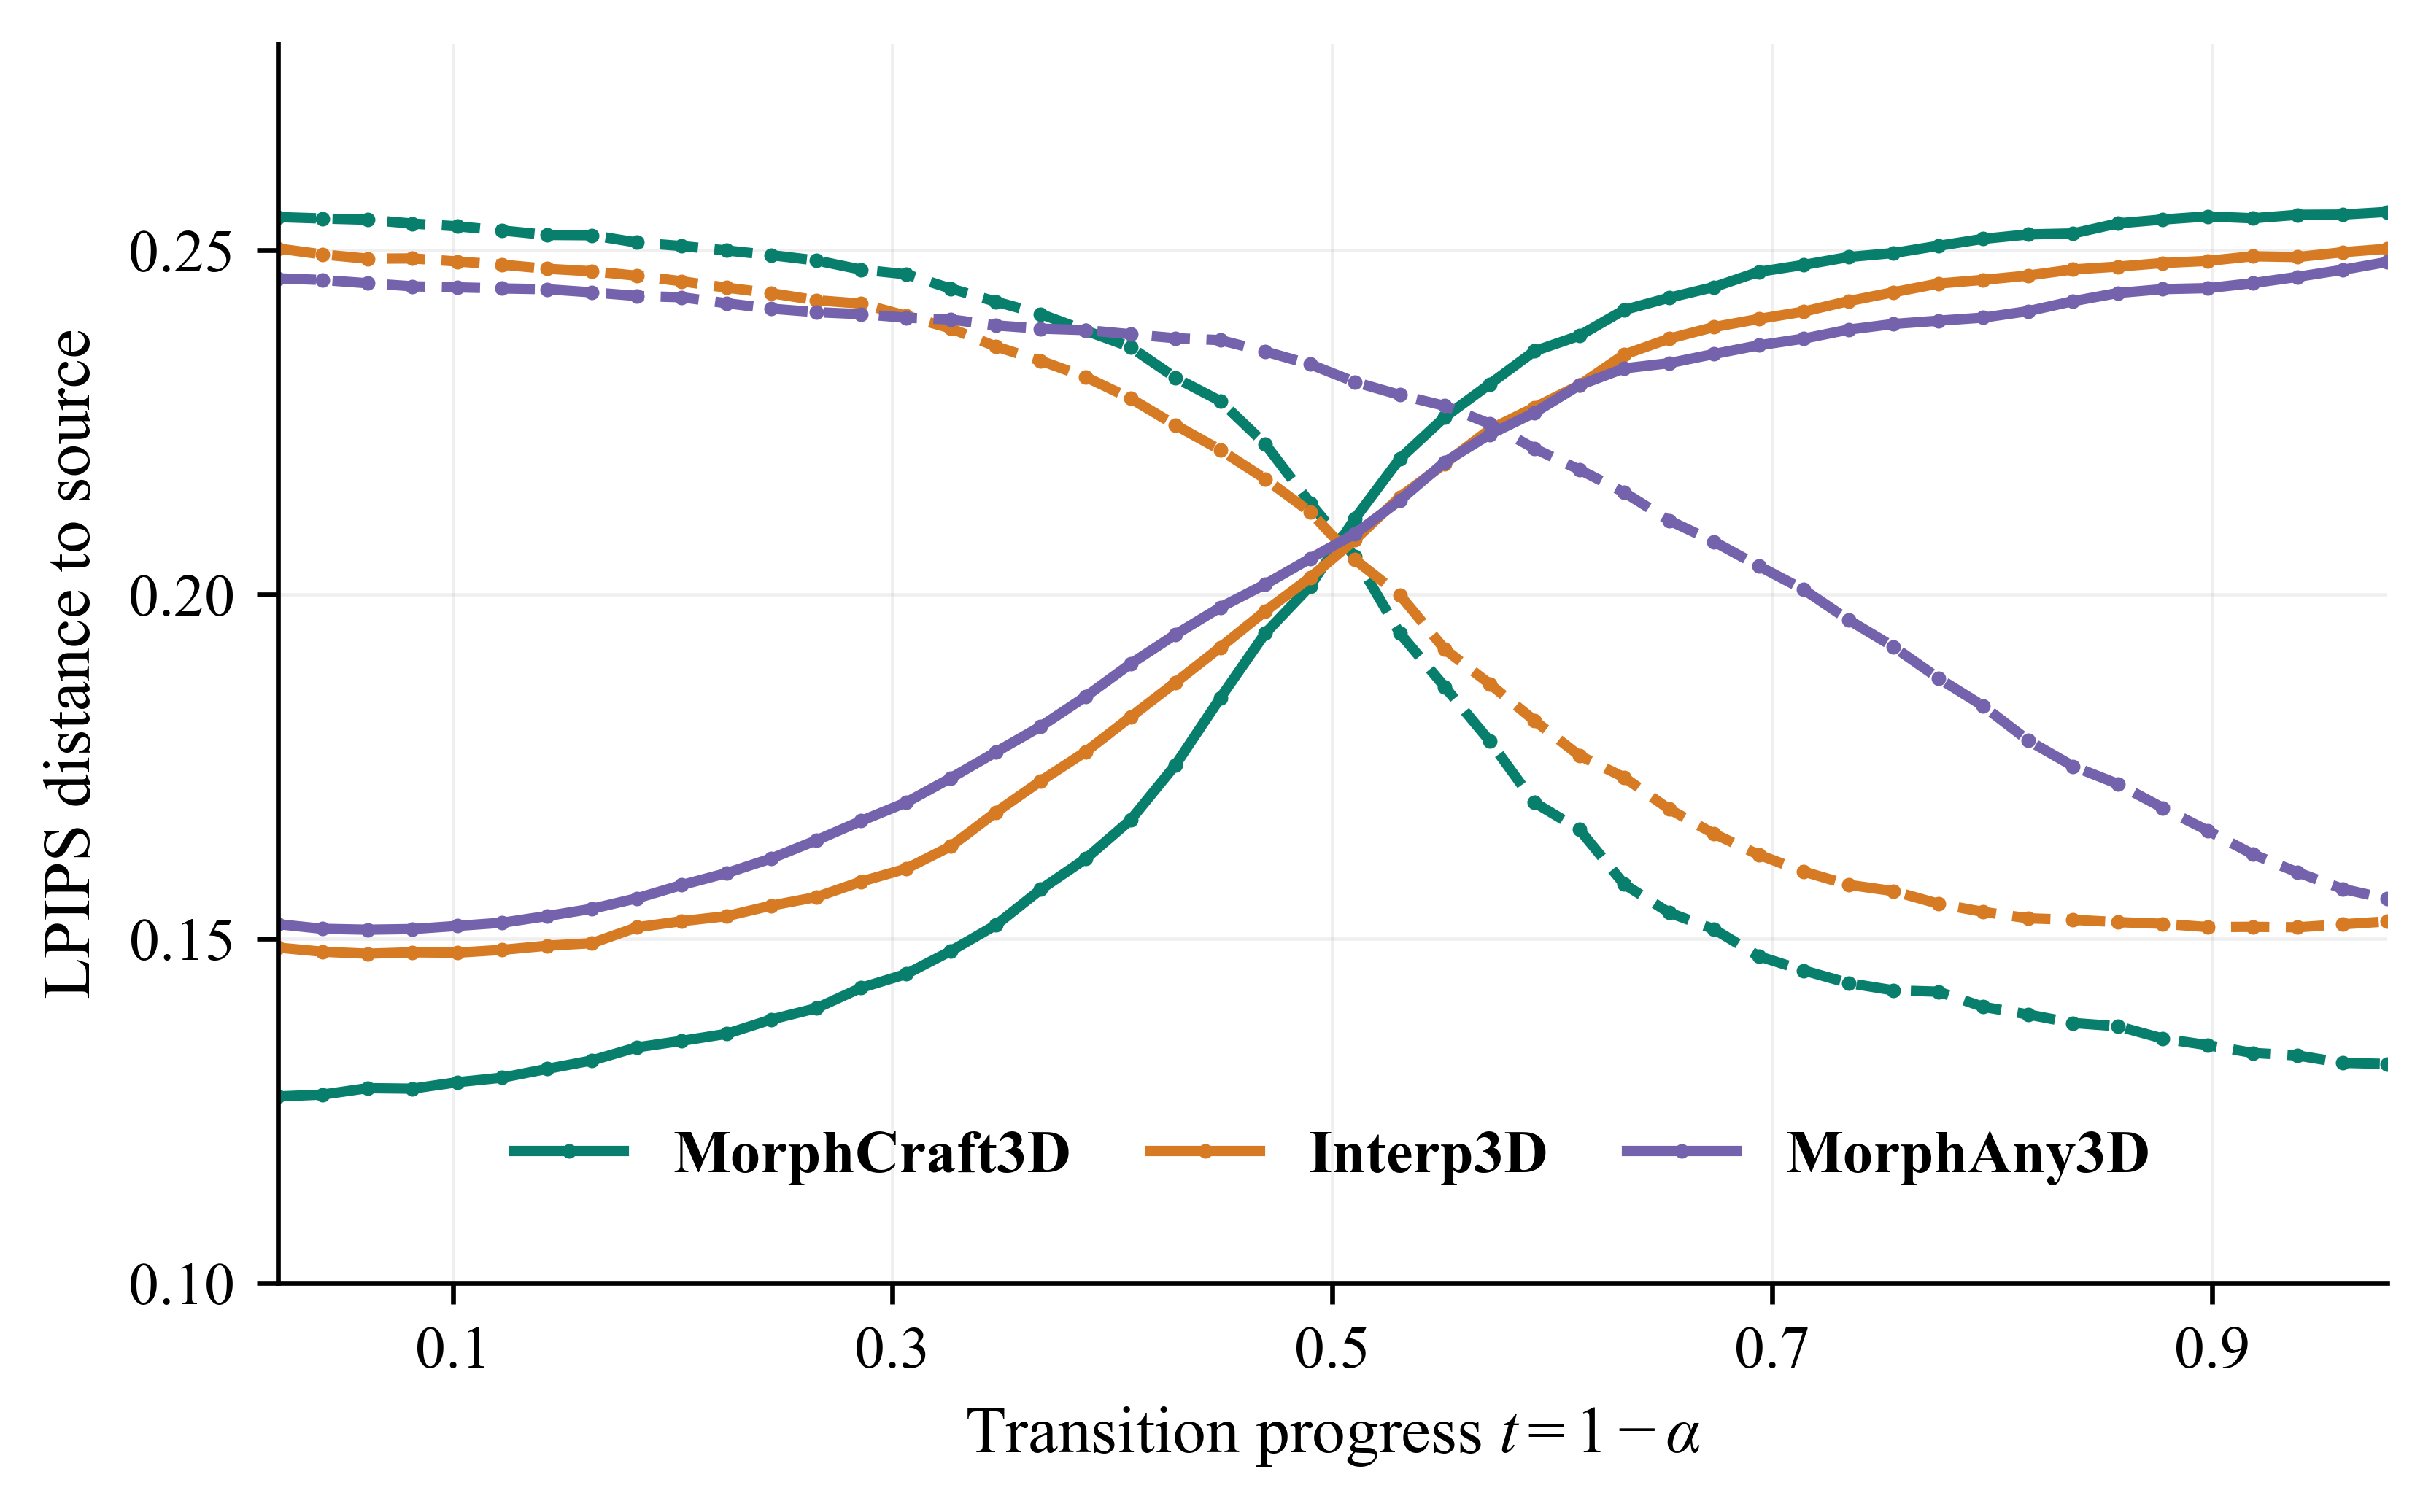
\includegraphics[width=\columnwidth]{figures/endpoint_distances_50.png}
%     \caption{\textbf{Perceptual distances to both sources.}
%     Solid and dashed curves show LPIPS distances to the first and second source, respectively. Colors identify the methods. Each curve averages 64 matched views over 50 object pairs and includes 48 generated intermediates. Canonical endpoints are omitted, with no connecting segments to $t=0$ or $t=1$.}
%     \label{fig:distances50}
% \end{figure}

% To examine this limitation, Figure~\ref{fig:distances50} shows how the perceptual distances from both sources evolve during morphing. Ideally, the distance from the first source should increase while that from the second decreases, with both curves intersecting near the midpoint. However, existing methods exhibit different behaviors. MorphAny3D produces asymmetric curves whose intersection is shifted from the center. Interp3D exhibits a more balanced profile, while our method shows a similar central intersection with greater separation between the source distances near the endpoints. These differences highlight the need to explicitly measure how the transition moves away from one source and approaches the other.

%SPE compares perceptual distances to both sources with linear reference profiles. %Given the multiple possible trajectories between two objects, these profiles provide a common reference for comparison.
% Since two objects do not define a unique morphing trajectory, we do not assume that perceptual linearity is the only valid behavior. Instead, we use it as a simple and interpretable reference in which the interpolation coefficient corresponds to a uniform progression between the sources.

% SPE compares perceptual distances to both sources. Let $M(\alpha)$ denote the generated asset at coefficient $\alpha\in[0,1]$, with $\alpha=1$ corresponding to $S_1$ and $\alpha=0$ to $S_2$. Let $d(\cdot,\cdot)$ denote LPIPS~\cite{zhang2018lpips} averaged over matched camera views. We define the normalized source-distance profiles as
% \begin{equation}
%  r_i(\alpha)=
%  \frac{d(M(\alpha),S_i)}{d(S_1,S_2)},
%  \qquad i\in\{1,2\}.
% \end{equation}
% The linear reference profiles are $1-\alpha$ for $S_1$ and $\alpha$ for $S_2$. We measure their squared deviation as
% \begin{equation}
%  \begin{aligned}
%  q(\alpha)=\frac12\big[
%  &(r_1(\alpha)-(1-\alpha))^2+(r_2(\alpha)-\alpha)^2\big].
%  \label{eq:profile_error}
%  \end{aligned}
% \end{equation}
% SPE aggregates this deviation along the trajectory:
% \begin{equation}
%  \spe=\sqrt{\int_0^1 q(\alpha)\,d\alpha}.
%  \label{eq:spe}
% \end{equation}
% We approximate the integral using the trapezoidal rule over the sampled coefficients and average the resulting scores across object pairs. Lower SPE indicates closer agreement with the reference progression.

SPE evaluates how closely the perceptual distances between generated assets and their sources align with the interpolation coefficient. Let $M(\alpha)$ denote the generated asset at coefficient $\alpha\in[0,1]$, where $\alpha=1$ corresponds to $S_1$ and $\alpha=0$ to $S_2$. We use LPIPS~\cite{zhang2018lpips}, averaged over matched camera views, as the perceptual distance $d(\cdot,\cdot)$. The distances to each source are normalized by the distance between the two sources:
\begin{equation}
 r_i(\alpha)=
 \frac{d(M(\alpha),S_i)}{d(S_1,S_2)},
 \qquad i\in\{1,2\}.
\end{equation}

For each interpolation coefficient, the target normalized distances to $S_1$ and $S_2$ are $1-\alpha$ and $\alpha$, respectively. We quantify the deviation from these targets as
\begin{equation}
 \begin{aligned}
 q(\alpha)=\frac12\big[
 &(r_1(\alpha)-(1-\alpha))^2+(r_2(\alpha)-\alpha)^2\big].
 \label{eq:profile_error}
 \end{aligned}
\end{equation}
SPE aggregates this deviation over the interpolation trajectory:
\begin{equation}
 \spe=\sqrt{\int_0^1 q(\alpha)\,d\alpha}.
 \label{eq:spe}
\end{equation}
We approximate the integral using the trapezoidal rule over the sampled coefficients and average the resulting scores across object pairs. Lower SPE indicates closer agreement with the reference progression.
% Figure~\ref{fig:epre_profile} shows how the squared profile error varies along the transition. Our method achieves lower errors over most of the trajectory, particularly near the endpoints, while remaining comparable to Interp3D around the midpoint. Table~\ref{tab:standard} reports the aggregated EPRE scores under two evaluation protocols. The Interp Protocol uses five intermediate states, whereas the Dense Protocol evaluates 48 intermediates, providing a more detailed assessment of progression throughout the transition.